% \subsection*{Abstract}

  \noindent Studies in the field of synthetic biology make constant additions to existing repositories of biological circuits, as well as to the theoretical understanding of their capabilities.
  Although many synthetic gene networks have been demonstrated able to perform computations using biomolecules, until recently the majority of such models were engineered to implement the functionality of single reusable circuit parts.
  \citet{originals} have proposed a network capable of multiple functions, allowing for the selection of three different behaviours in a programmable fashion.
  This work provides a reference open-source implementation which is used to replicate that study.


\section{Introduction}

  The field of biomolecular computing -- and \acs{dna}-based computing in particular -- has advanced remarkably over the last years \cite{analog}.
  There are numerous designs of biological parts which implement the behavior of digital logic gates \supercite{async}, continuous-time systems \supercite{analog}, oscillators \supercite{repressilator}, memory components \supercite{async}, asynchronous circuits \supercite{async} and so on.
  Such recent developments allow one to consider the possibility of exploting biologically derived materials and their aspects of massive parallelism and self-replication to build practical computing systems on biological \textit{substrata} \cite{youtuber}.

  Amidst forward-engineered biochemical systems, genetic oscillators have been a focus of research as they are required for the correct operation of sequential circuits and can also provide persistent periodic \textit{stimulus} to other regulatory networks which may rely on them \cite{ingalls}.
  Genetic switches present another functionality specially useful to digital logic: the ability to toggle between on or off states by either activating or repressing the expression of a certain gene makes them equivalent to a cellular memory unit \cite{youtuber}.
  One study\supercite{clock} has shown that combining an oscillator with a toggle switch under certain circumstances will result in the generation of a clock-like near square wave signal.

  \citet{originals} presented the \textit{in silico} design of a novel genetic regulatory network which performs frequency division on an oscillating input.
  During experiments, that model was discovered able to behave not only as a frequency multiplier, but also as a self-induced oscillator or toggle switch.
  We believe such multi-functionality may lead to the creation of reusable programmable components in biological computing and this has led to the reproduction of the simulations described in that paper on an open-source implementation of the aforementioned model.


\section{Methods}

  The multi-functional synthetic gene network and its dynamics are wholly described in the original study.
  Supplementary material contains the full \ac{ode} system under mass-action kinetics with Hill functions used to represent activation and repression of genetic promoters.
  The \ac{qssa} exploited to derive the reduced model considered in simulations is also provided, together with all reaction parameterisation and initial state of each experiment.
  These factors allowed for an easy replication of the model, even without direct reference to the original source code or usage of the proprietary tools which were employed.
  All numerical simulations were performed in Octave (version 5.1.0) using Euler's method with a fixed step size of 60 seconds.
  This is justified based on the duration of experiments, the shortest of which take at least four days (virtual simulated time) in order to observe a couple of periods on the oscillating output of the frequency divider.

  We borrow the network's parameters and mathematical description from the original paper to reproduce each of the hereby presented simulations.
  Every deterministic experiment was carried in two systems: one considering the full set of \ac{ode}s and another with the \ac{qssa} approximation that is used throughout that study.
  We present a brief comparison of these models' quantitative results and highlight their differences.
  While stochastic experiments are only briefly mentioned on the main text, more details can be found inside supporting information documents provided by \citet{originals}.
  The \ac{cles} described therein were implemented with Gaussian noise being generated through the use of built-in Octave functions.


\section{Results}

  \subsection{Frequency Divider}

    Although the network is said to be a frequency multiplier, it actually performs frequency division as concentrations of repressor proteins oscillate in one half of the input frequency or, equivalently, with a period that is twice as long.
    This behaviour can be observed by feeding the model with a continuously oscillating input -- this would be often the case considering existing genetic oscillators -- but also works with square waves, as shown in Figure \ref{fig.freqdiv-square-zero}.

    \begin{figure}[!htb]
      \centering
      \begin{subfigure}[t]{0.4\textwidth}
        \centering
        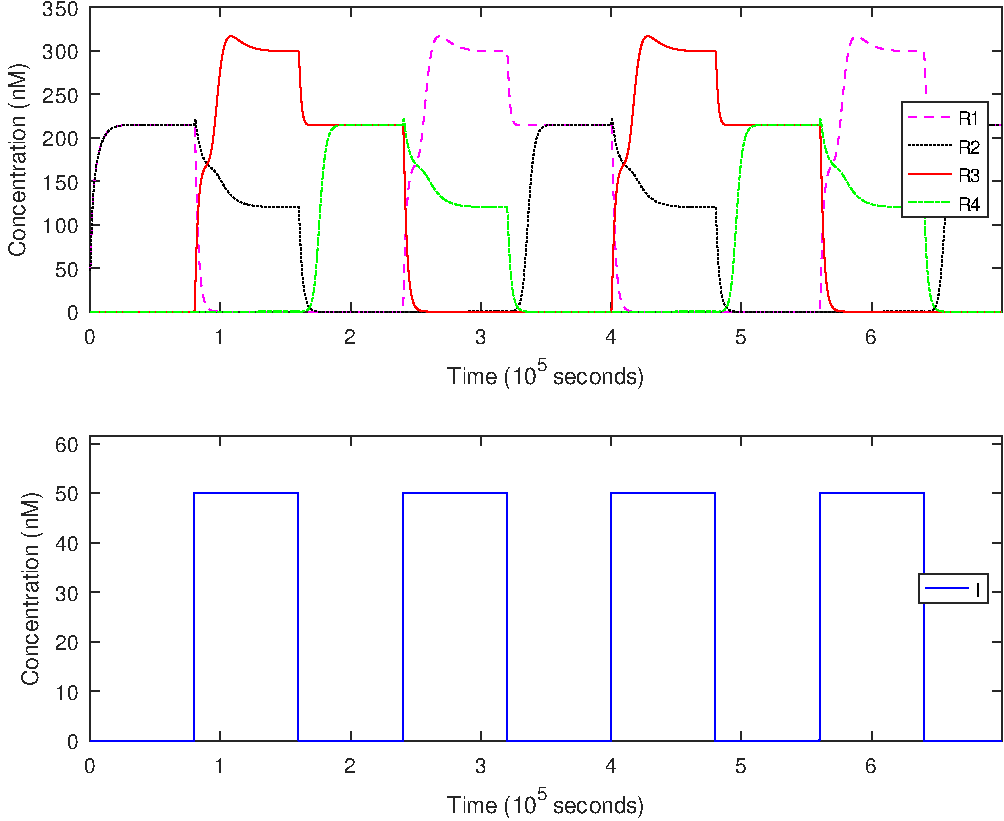
\includegraphics[width=\linewidth]{freqdiv-square}
        \caption{Input signal is a square wave with amplitude of \SI{50}{\nano M}, period of $1.6 \times 10^5$ seconds and a duty cycle of $50\%$. The period-doubling effect is highlighted by repressor R3.}
        \label{fig.freqdiv-square}
      \end{subfigure}
      \hspace{1em}
      \begin{subfigure}[t]{0.4\textwidth}
        \centering
        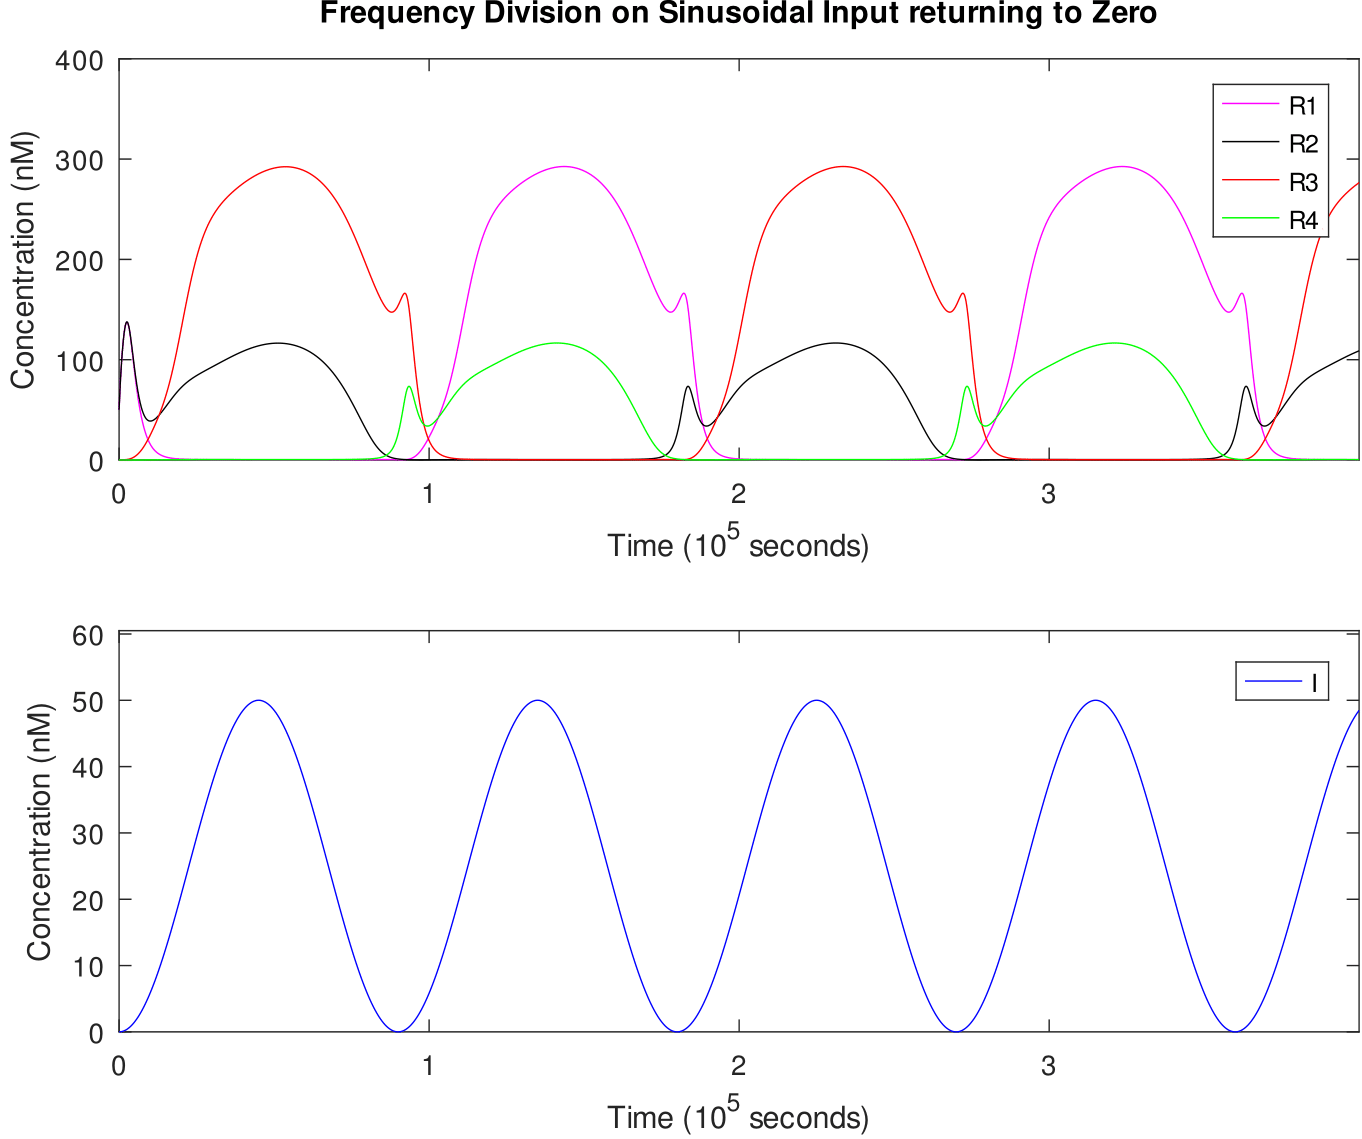
\includegraphics[width=\linewidth]{freqdiv-zero}
        \caption{Sinusoidal input with \SI{50}{\nano M} amplitude and period of $0.9 \times 10^5$ seconds with valleys reaching zero concentration.}
        \label{fig.freqdiv-zero}
      \end{subfigure}
      \caption{\textbf{Frequency division for discrete and continuous inputs.} Initial conditions are $R1 = R2 = 50nM$ and $R3 = R4 = 0nM$. Reaction parameters from the reference text are used.}
      \label{fig.freqdiv-square-zero}
    \end{figure}

    \begin{figure}[!htb]
      \centering
      \begin{subfigure}[t]{0.45\textwidth}
        \centering
        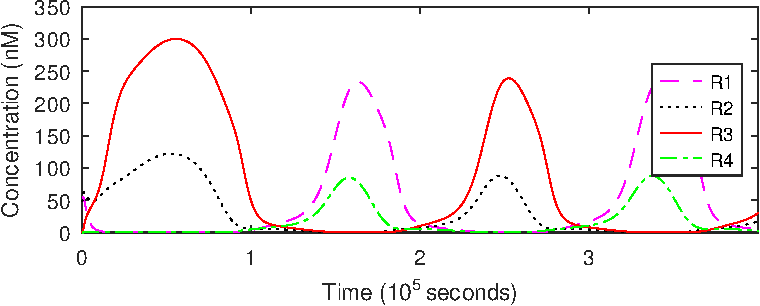
\includegraphics[width=\linewidth]{freqdiv-full}
        \caption{}
        \label{fig.freqdiv-full}
      \end{subfigure}
      \hspace{1em}
      \begin{subfigure}[t]{0.45\textwidth}
        \centering
        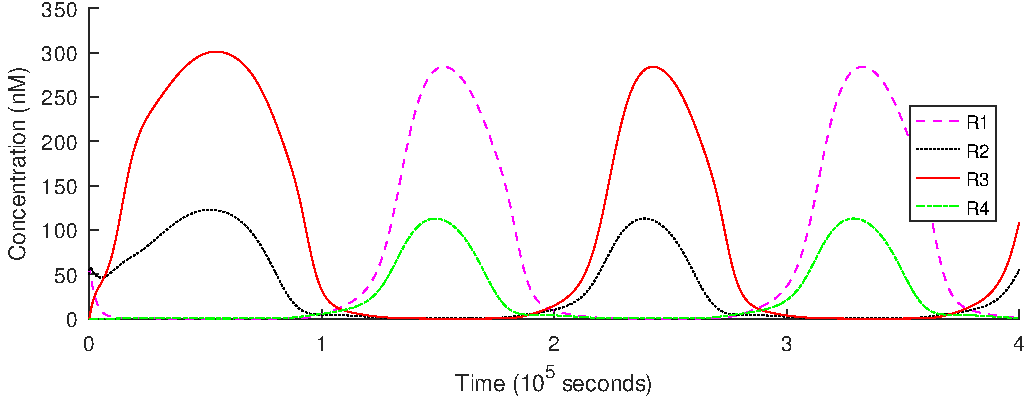
\includegraphics[width=\linewidth]{freqdiv-qssa}
        \caption{}
        \label{fig.freqdiv-qssa}
      \end{subfigure}
      \caption{\textbf{Comparing frequency division outputs between full and reduced models.} Initial conditions are $R1 = R2 = 50nM$, $R3 = R4 = 0nM$ and reaction parameters from the reference text are used. In both simulations the input signal has an amplitude of \SI{50}{\nano M}, period is $0.9 \times 10^5$ seconds and minimum concentrations reached are \SI{6}{\nano M}.}
      \label{fig.freqdiv-sinusoidal}
    \end{figure}

    With a sinusoidal input, output signals from the \ac{qssa} model have constant amplitude, whereas in the full model the first concentration peak of proteins R2 and R3 are higher than the following ones.
    This suggests \acs{mrna} reactions stabilize quicker in the first $10^5$ seconds and thus the approximation is more accurate at those instants.
    After that moment, however, the reduced model exhibits a persistent error in relation to the complete one, which can be observed by comparing concentration levels reached during oscillation peaks in Figures \ref{fig.freqdiv-full} and \ref{fig.freqdiv-qssa}.

    In those simulations, while R1 and R4 concentrations in the full model reach \textit{maxima} valued at \SI{238.29}{\nano M} and \SI{87.62}{\nano M} respectively, the reduced model (again, this is the one presented in the original paper) goes up to \SI{283.96}{\nano M} and \SI{113.05}{\nano M} for each of these proteins.
    Peak values of R3 follow R1 closely and the same happens with R2 and R4.
    This offset distinguishing the two models happens because the \ac{qssa} used to derive the reduced \ac{ode} system considers a separation of time-scales between reactions which regulate \acs{mrna} production and those which describe protein translation.
    In the approximation, the former reactions are assumed to reach equilibrium instantaneously relative to the latter.
    Thus, the difference is a consequence of the fact that the original model maintains itself in a dynamic state that never actually reaches equilibrium, as it perpetually oscillates \cite{ingalls}.

    \begin{figure}[!htb]
      \centering
      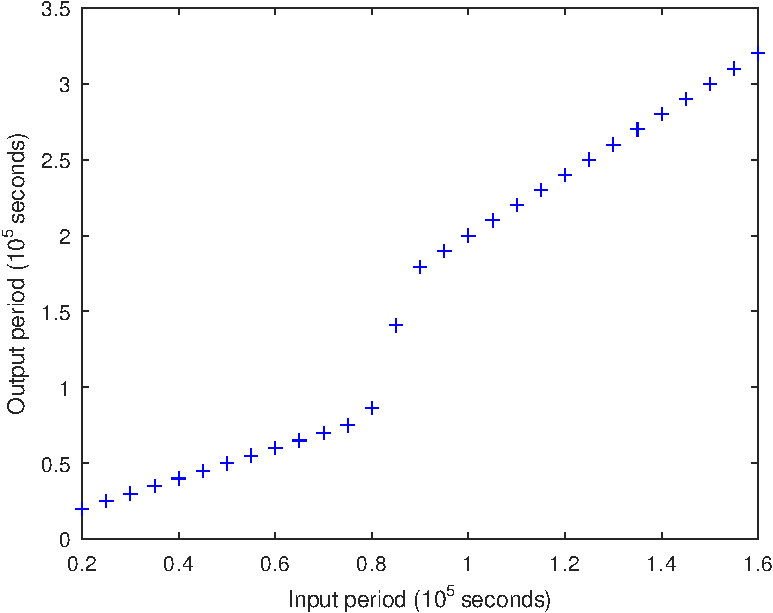
\includegraphics[width=0.65\textwidth]{freqdiv-period}
      \caption{\textbf{Locating the period-doubling bifurcation.} Output frequency was detected by measuring the distance between peaks of R1 concentration. Other than input frequency and simulation length (each run was configured to take as long as five times the input period), parameters are the same as in Figure \ref{fig.freqdiv-sinusoidal}.}
      \label{fig.freqdiv-period}
    \end{figure}

    As mentioned in the original study, the frequency division functionality can only be observed after a specific period threshold.
    We ran simulations under the full model on a range of input frequencies and found the period-doubling bifurcation to be located near values of $8 \times 10^4$ seconds ($\sim 22.22$ hours).
    Results are shown in Figure \ref{fig.freqdiv-period}.
    These diverge from the reference work, where it is stated that this threshold could be observed at input periods of $\sim 27500$ seconds ($\sim 8$ hours).
    This confirms the proposed network is better suited to interfacing with long-period oscillators, although a more in-depth parameter exploration is needed in order to verify its compatibility with higher frequencies.


  \subsection{Bifurcation Analysis}

    \citet{originals} discovered the model's multiple extra functionalities by verifying different behaviours could be attained by holding input concentration constant at specific ranges.
    Six bifurcation analysis experiments were reproduced, where reaction parameters and input levels are the same as in the original work and initial conditions used are $R1=R2=0nM$ and $R3=R4=50nM$ for simulations $1b$ and $4c_{2}$ and $R1=R2=50nM$ and $R3=R4=0nM$ for all others.
    The original text states simulations labeled $4c_{1}$ and $1b$ use the same initial conditions as $4c_{2}$ and $1a$ respectively.
    We believe these were typographical errors, as such settings would lead the mentioned experiments to be exactly the same under deterministic semantics and this is not what is exhibited.

    \begin{figure}[!htb]
      \centering
      \begin{subfigure}[t]{0.4\textwidth}
        \centering
        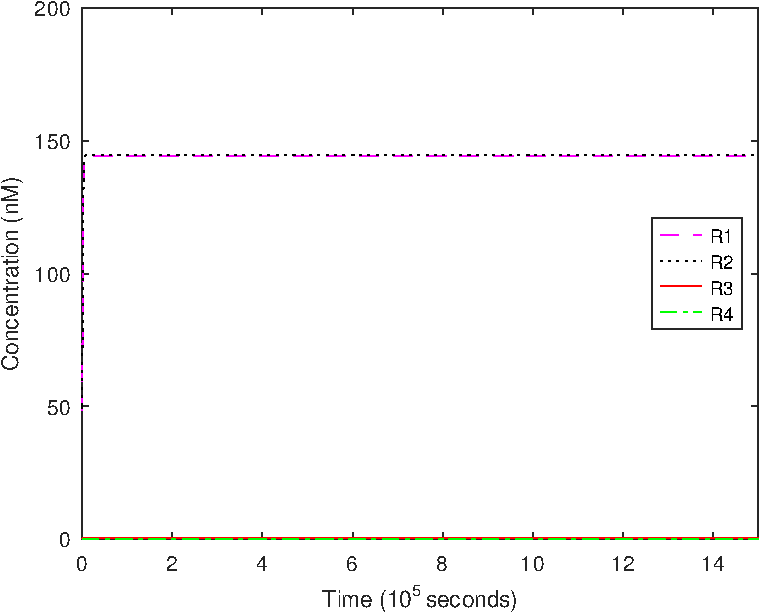
\includegraphics[width=\linewidth]{bifurcation-1a}
        \caption{\textbf{Experiment $1a$.} Protein concentrations are initially set to $R1 = R2 = 50nM$ and $R3 = R4 = 0nM$.}
        \label{fig.bifurcation-1a}
      \end{subfigure}
      \hspace{1em}
      \begin{subfigure}[t]{0.4\textwidth}
        \centering
        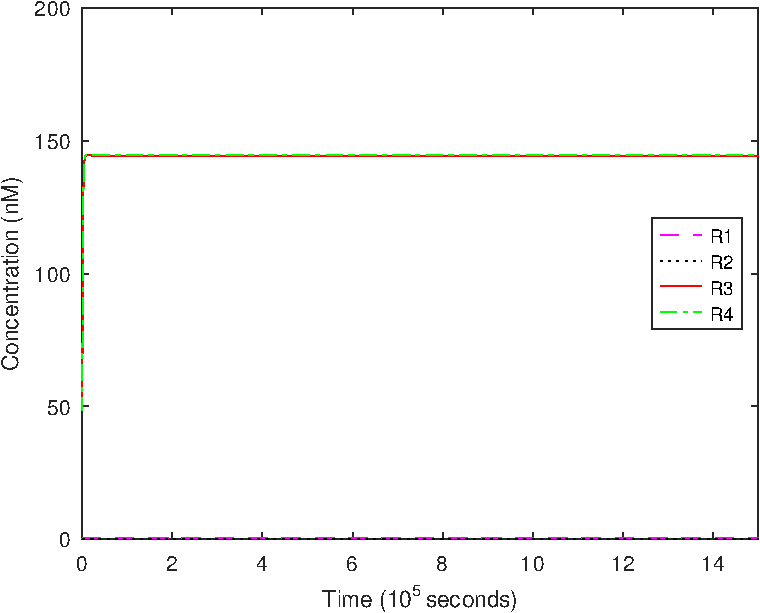
\includegraphics[width=\linewidth]{bifurcation-1b}
        \caption{\textbf{Experiment $1b$.} Protein concentrations are initially set to $R1 = R2 = 0nM$ and $R3 = R4 = 50nM$.}
        \label{fig.bifurcation-1b}
      \end{subfigure}
      \caption{\textbf{Low concentration bistable behaviour.} $I = 0.1 nM$}
      \label{fig.bifurcation-1}
    \end{figure}

    \begin{figure}[!htb]
      \centering
      \begin{subfigure}[t]{0.45\textwidth}
        \centering
        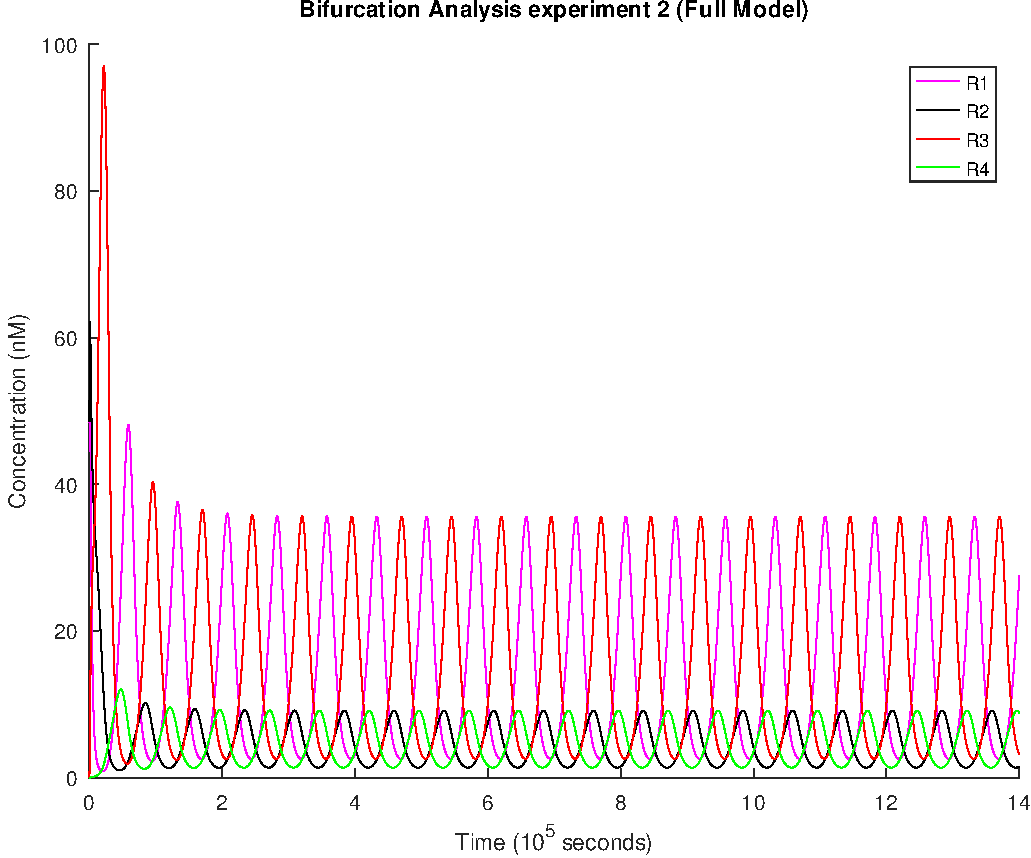
\includegraphics[width=\linewidth]{bifurcation-2-full}
        \caption{}
        \label{fig.bifurcation-2-full}
      \end{subfigure}
      \hspace{1em}
      \begin{subfigure}[t]{0.45\textwidth}
        \centering
        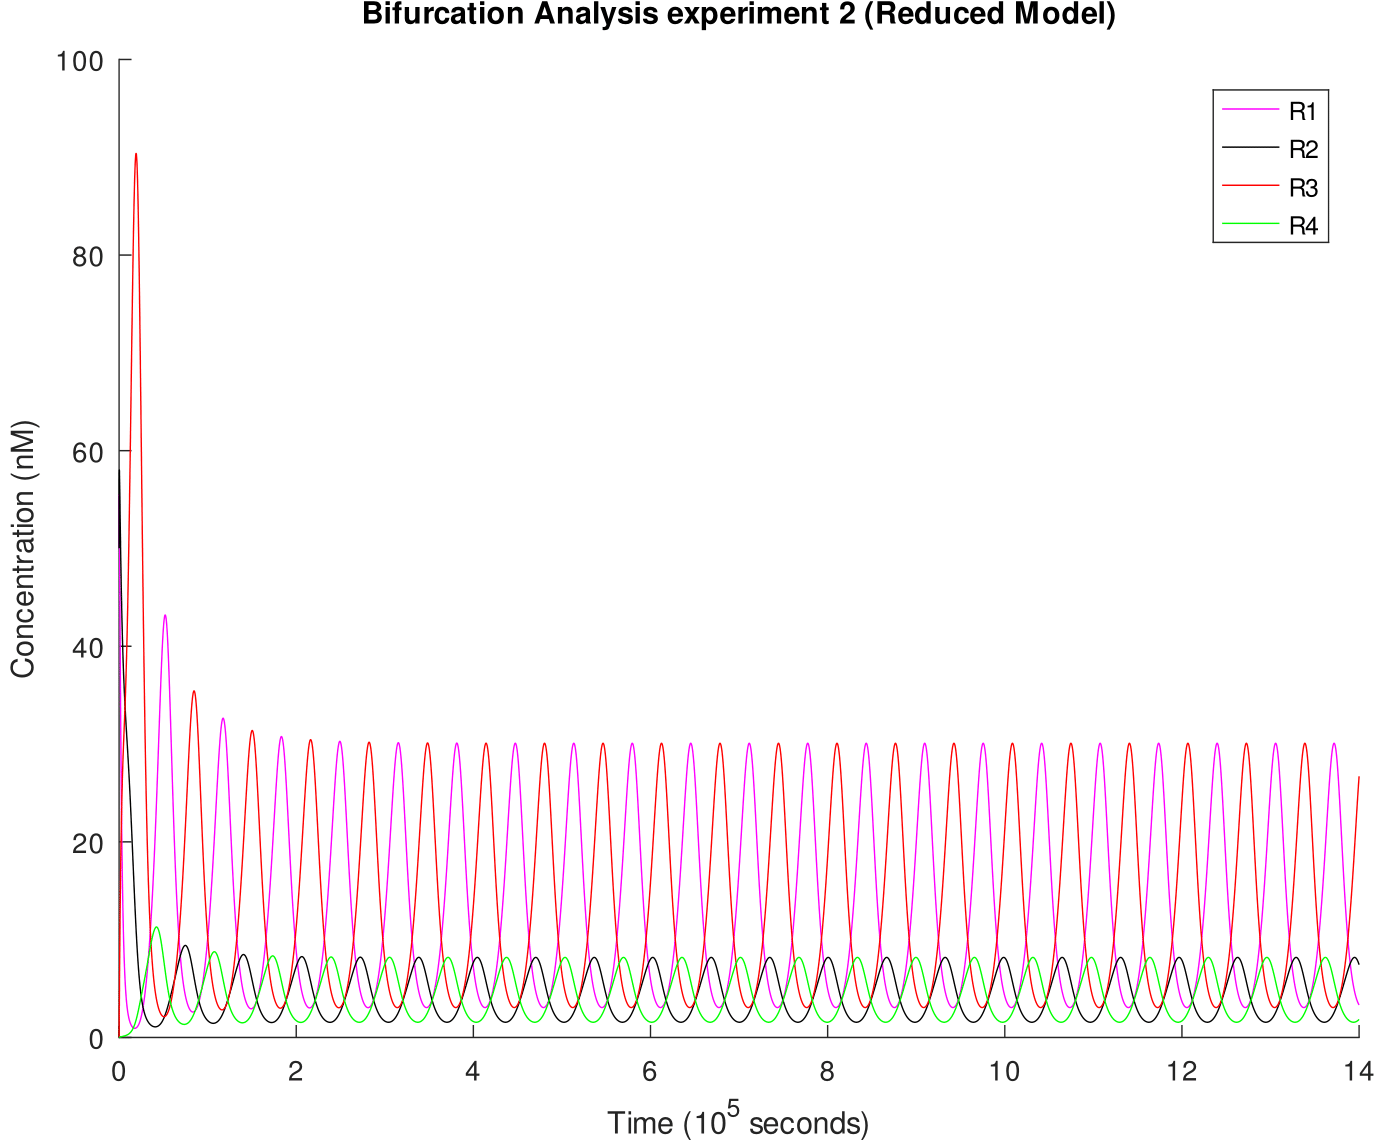
\includegraphics[width=\linewidth]{bifurcation-2-qssa}
        \caption{}
        \label{fig.bifurcation-2-qssa}
      \end{subfigure}
      \caption{\textbf{Comparing oscillation amplitude in experiment $2$.} Initial conditions are $R1 = R2 = 50nM$, $R3 = R4 = 0nM$ and input is held at a constant level of \SI{5}{\nano M}.}
      \label{fig.bifurcation-2}
    \end{figure}

    Once again, oscillation amplitude differs between models, with R1 and R4 each peaking at \SI{35.60}{\nano M} and \SI{9.16}{\nano M} in the complete system (Figure \ref{fig.bifurcation-2-full}) while going up to \SI{30.08}{\nano M} and \SI{8.18}{\nano M} in the \ac{qssa} reduction (Figure \ref{fig.bifurcation-2-qssa}).
    Other experiments do not present such significant offset.

    \begin{figure}[!htb]
      \centering
      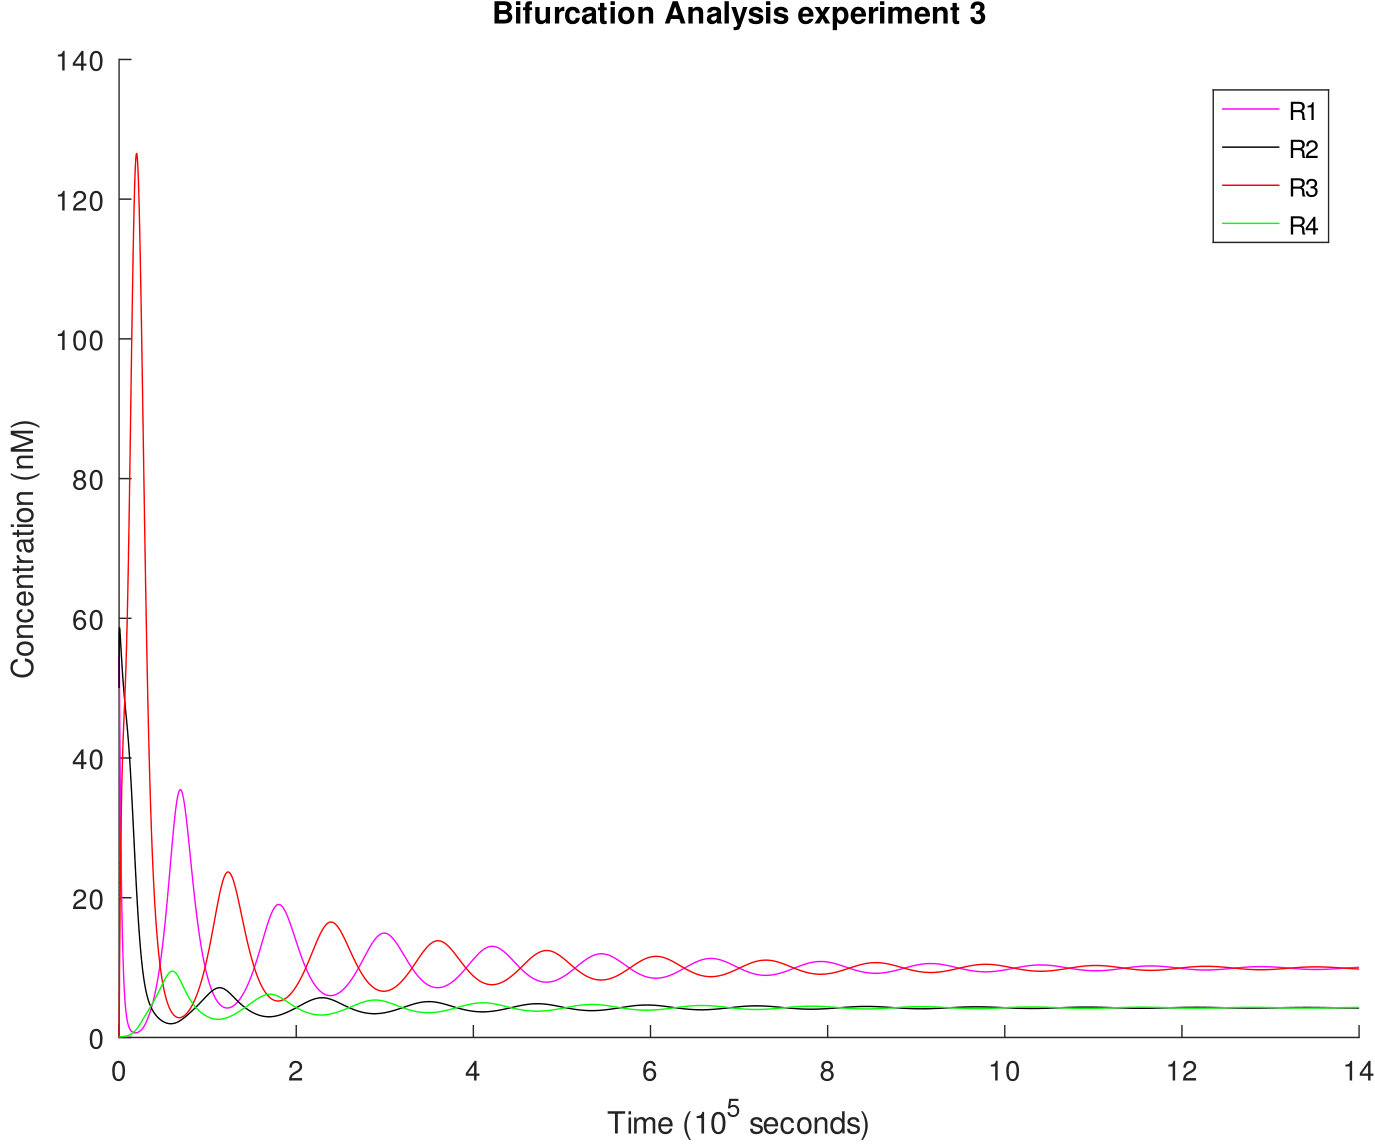
\includegraphics[width=0.6\textwidth]{bifurcation-3}
      \caption{\textbf{Evidence for pitchfork bifurcation in experiment $3$.} $I = 7.5nM$.}
      \label{fig.bifurcation-3}
    \end{figure}

    \begin{figure}[!htb]
      \centering
      \begin{subfigure}[t]{0.45\textwidth}
        \centering
        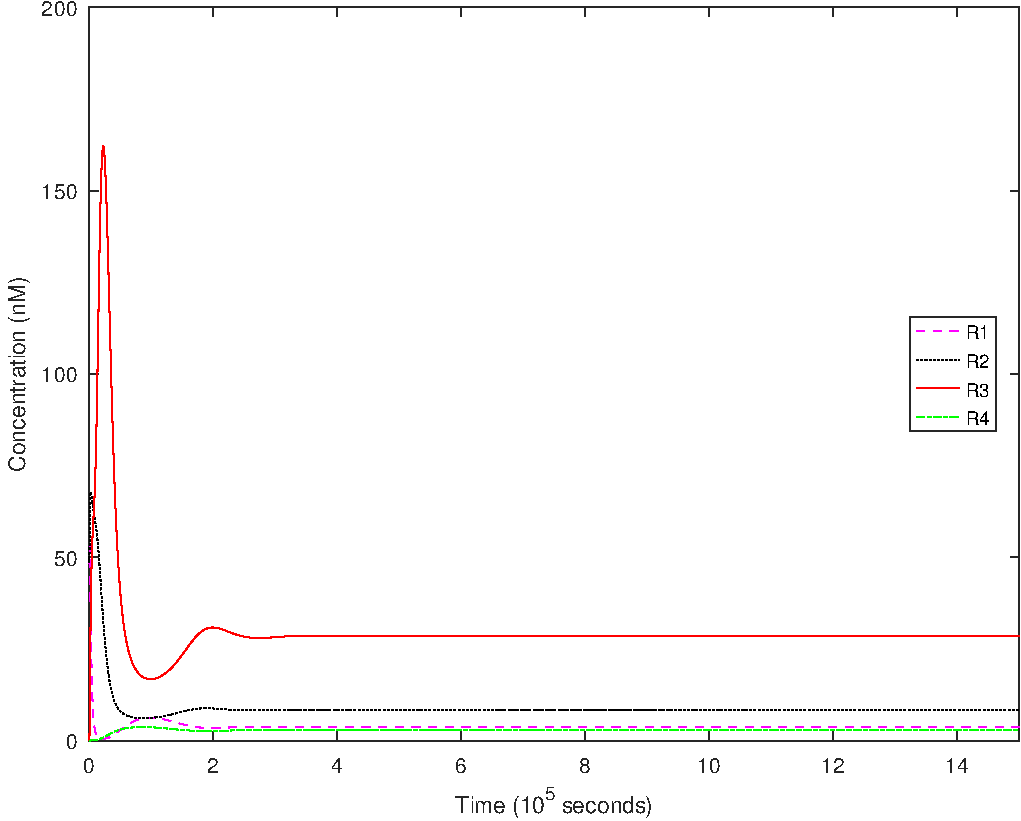
\includegraphics[width=\linewidth]{bifurcation-4c1}
        \caption{\textbf{Experiment $4c_{1}$.} Protein concentrations are initially set to $R1 = R2 = 50nM$ and $R3 = R4 = 0nM$.}
        \label{fig.bifurcation-4c1}
      \end{subfigure}
      \hspace{1em}
      \begin{subfigure}[t]{0.45\textwidth}
        \centering
        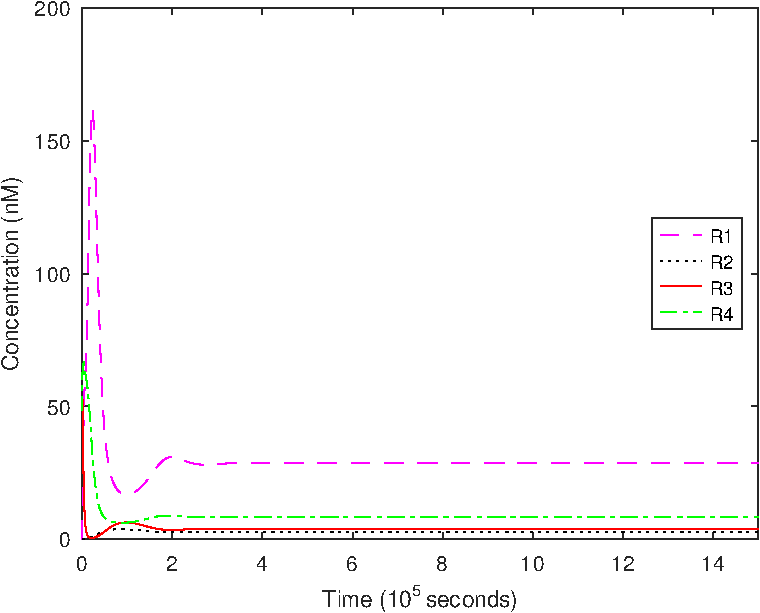
\includegraphics[width=\linewidth]{bifurcation-4c2}
        \caption{\textbf{Experiment $4c_{2}$.} Protein concentrations are initially set to $R1 = R2 = 0nM$ and $R3 = R4 = 50nM$.}
        \label{fig.bifurcation-4c2}
      \end{subfigure}
      \caption{\textbf{High concentration bistable behaviour.} $I = 10 nM$}
      \label{fig.bifurcation-4}
    \end{figure}


  \subsection{Self-induced Oscillator}

    We verified the network's oscillatory dynamics in the region between saddle-node and Hopf bifurcations by measuring its output period for each given input concentration level.
    Thus, the analysis presented in the original work was reproduced without further difficulties: results describe a relation with similar behaviour and the same near-vertical increase in period as input approaches the lower bistability region.
    This is presented in Figure \ref{fig.oscillator-astable}.

    \begin{figure}[!htb]
      \centering
      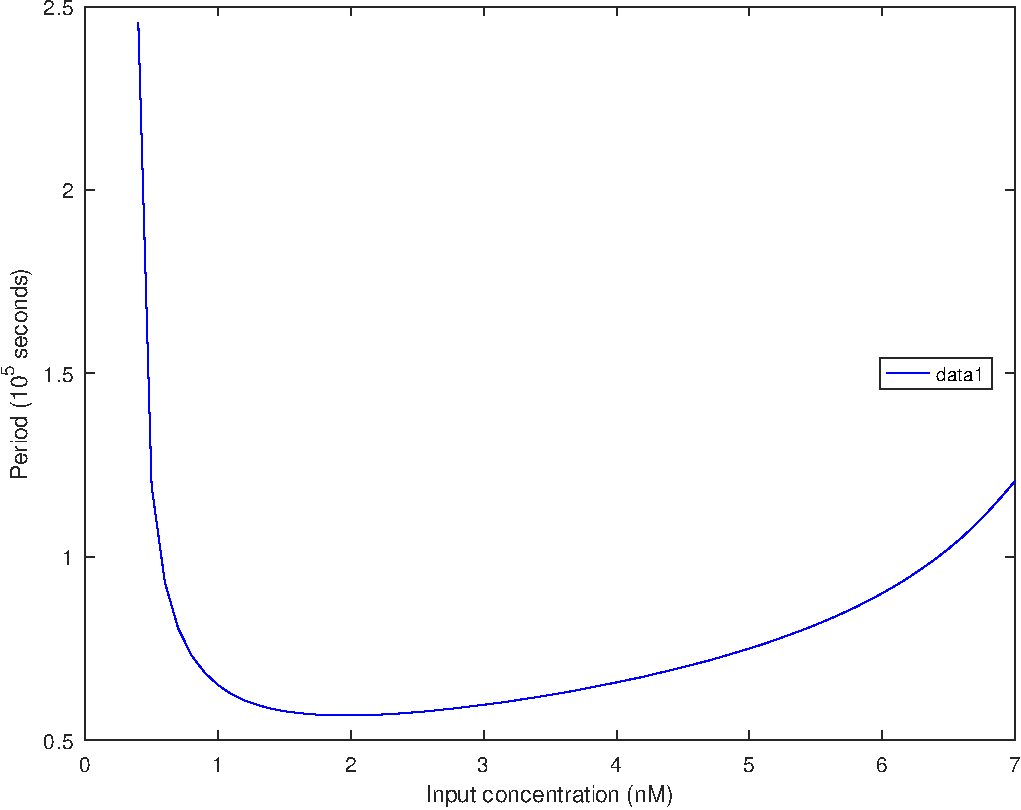
\includegraphics[width=0.9\textwidth]{oscillator-astable}
      \caption{\textbf{Analysing oscillatory dynamics.} Simulation configuration is the same as in Figure \ref{fig.bifurcation-2} except for input levels, which are held in the range $[0.4 \times 10^{-9}, 7 \times 10^{-9}]$. Output frequency was detected by measuring the distance between peaks of R1 concentration.}
      \label{fig.oscillator-astable}
    \end{figure}


  \subsection{Toggle Switch}

    As revealed during bifurcation analysis, the network exhibits bistability when input concentration is held outside the oscillatory range.
    Figures \ref{fig.switch-low} and \ref{fig.switch-high} illustrate simulations with the system being used as a toggle switch which is ``triggered'' by varying binding affinity of particular repressors.
    This set of experiments were exactly reproduced from the reference work, as all parameters are given, and no significant difference is found between reduced and full models.

    \begin{figure}[!htb]
      \centering
      \begin{subfigure}[t]{0.45\textwidth}
        \centering
        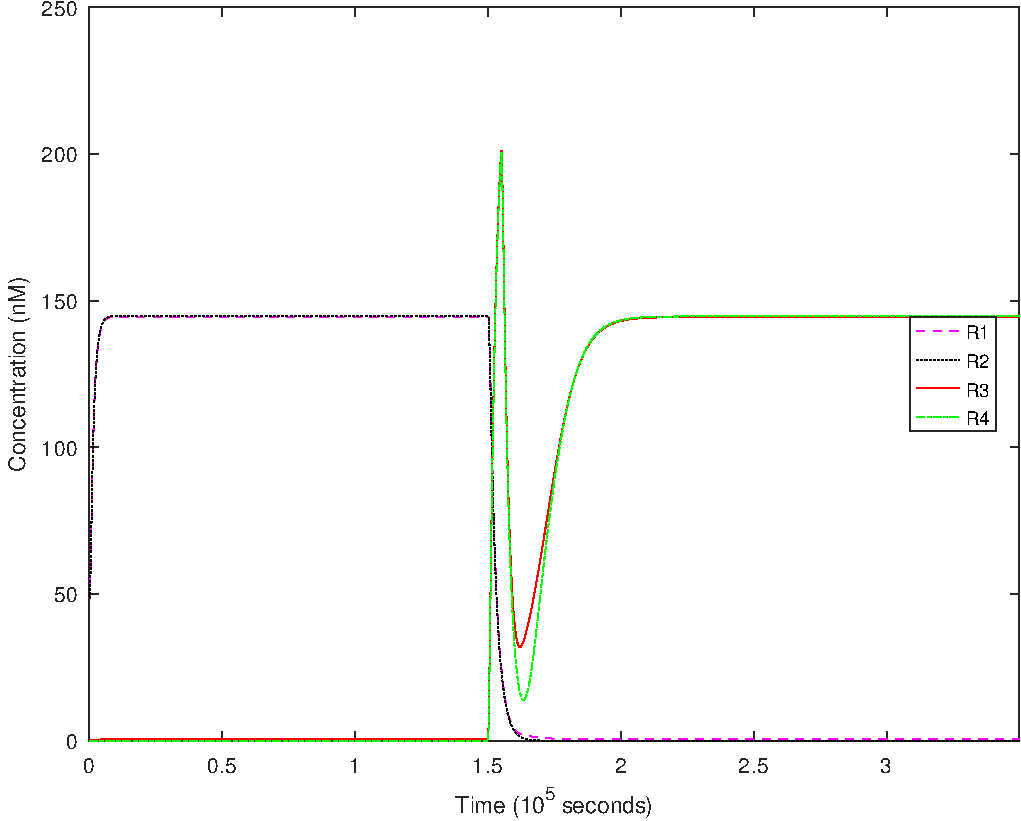
\includegraphics[width=\linewidth]{switch-A}
        \caption{Switch active state from R1 \& R2 to R3 \& R4. Initial conditions: $R1 = R2 = 50nM$, $R3 = R4 = 0nM$.}
        \label{fig.switch-A}
      \end{subfigure}
      \hspace{1em}
      \begin{subfigure}[t]{0.45\textwidth}
        \centering
        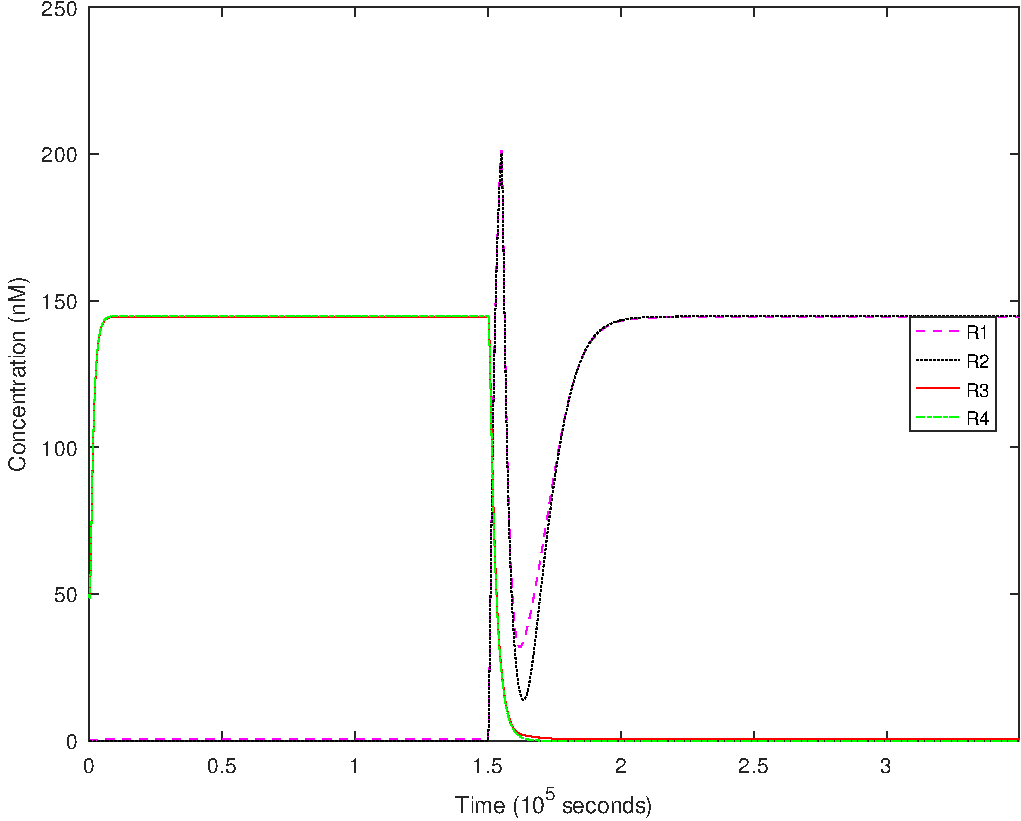
\includegraphics[width=\linewidth]{switch-B}
        \caption{Switch active state from R3 \& R4 to R1 \& R2. Initial conditions: $R1 = R2 = 0nM$, $R3 = R4 = 50nM$.}
        \label{fig.switch-B}
      \end{subfigure}
      \caption{\textbf{Toggle switch behaviour at low concentration.} $I = 0.1 nM$}
      \label{fig.switch-low}
    \end{figure}

    \begin{figure}[!htb]
      \centering
      \begin{subfigure}[t]{0.45\textwidth}
        \centering
        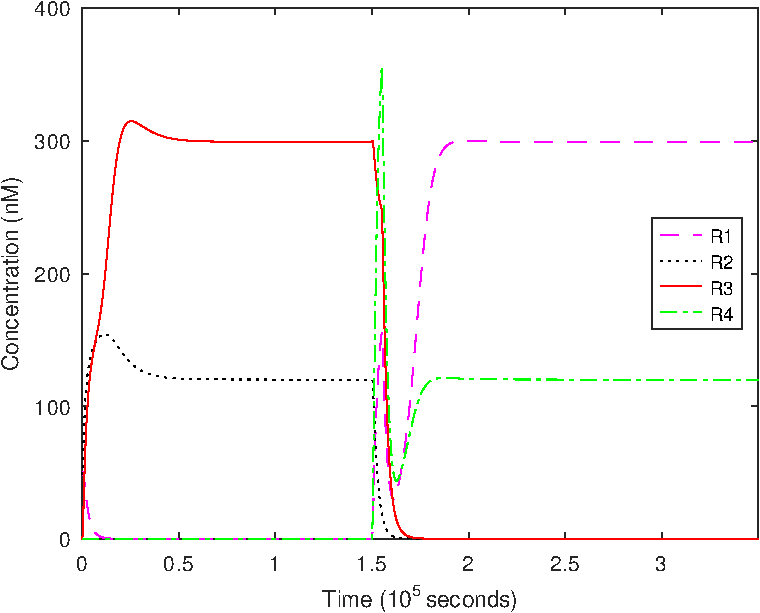
\includegraphics[width=\linewidth]{switch-C}
        \caption{Switch active state from R2 \& R3 to R1 \& R4. Initial conditions: $R1 = R2 = 50nM$, $R3 = R4 = 0nM$.}
        \label{fig.switch-C}
      \end{subfigure}
      \hspace{1em}
      \begin{subfigure}[t]{0.45\textwidth}
        \centering
        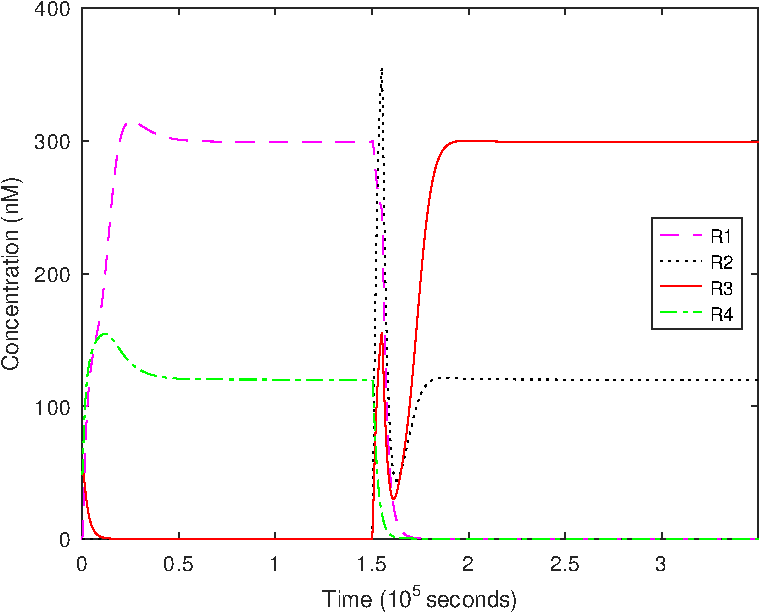
\includegraphics[width=\linewidth]{switch-D}
        \caption{Switch active state from R1 \& R4 to R2 \& R3. Initial conditions: $R1 = R2 = 0nM$, $R3 = R4 = 50nM$.}
        \label{fig.switch-D}
      \end{subfigure}
      \caption{\textbf{Toggle switch behaviour at high concentration.} $I = 50 nM$}
      \label{fig.switch-high}
    \end{figure}


  \subsection{Stochastic Simulations}

    We implemented the \ac{cles} shown in the related supporting information document provided by \citet{originals}, but it was not possible to verify similar results without modifications to the noise-inducing function.
    While original authors state the usage of Gaussian noise with zero mean and variance of 1, simply employing Octave's \code{randn} function -- which provides such a random distribution \cite{randn} -- proved being too noisy as stochastic fluctuations began dominating the model's behaviour.
    It was found through trial and error that downscaling random numbers by a factor of $s \in [\frac{1}{100}, \frac{1}{10}]$ (and consequently scaling variance by $s^2$) would bring results closer to what is seen in the reference work.

    Wishing to increase reproductibility, stochastic simulations mentioned in this text were performed with a hardcoded random seed for the noise-generating function.

    \begin{figure}[!htb]
      \centering
      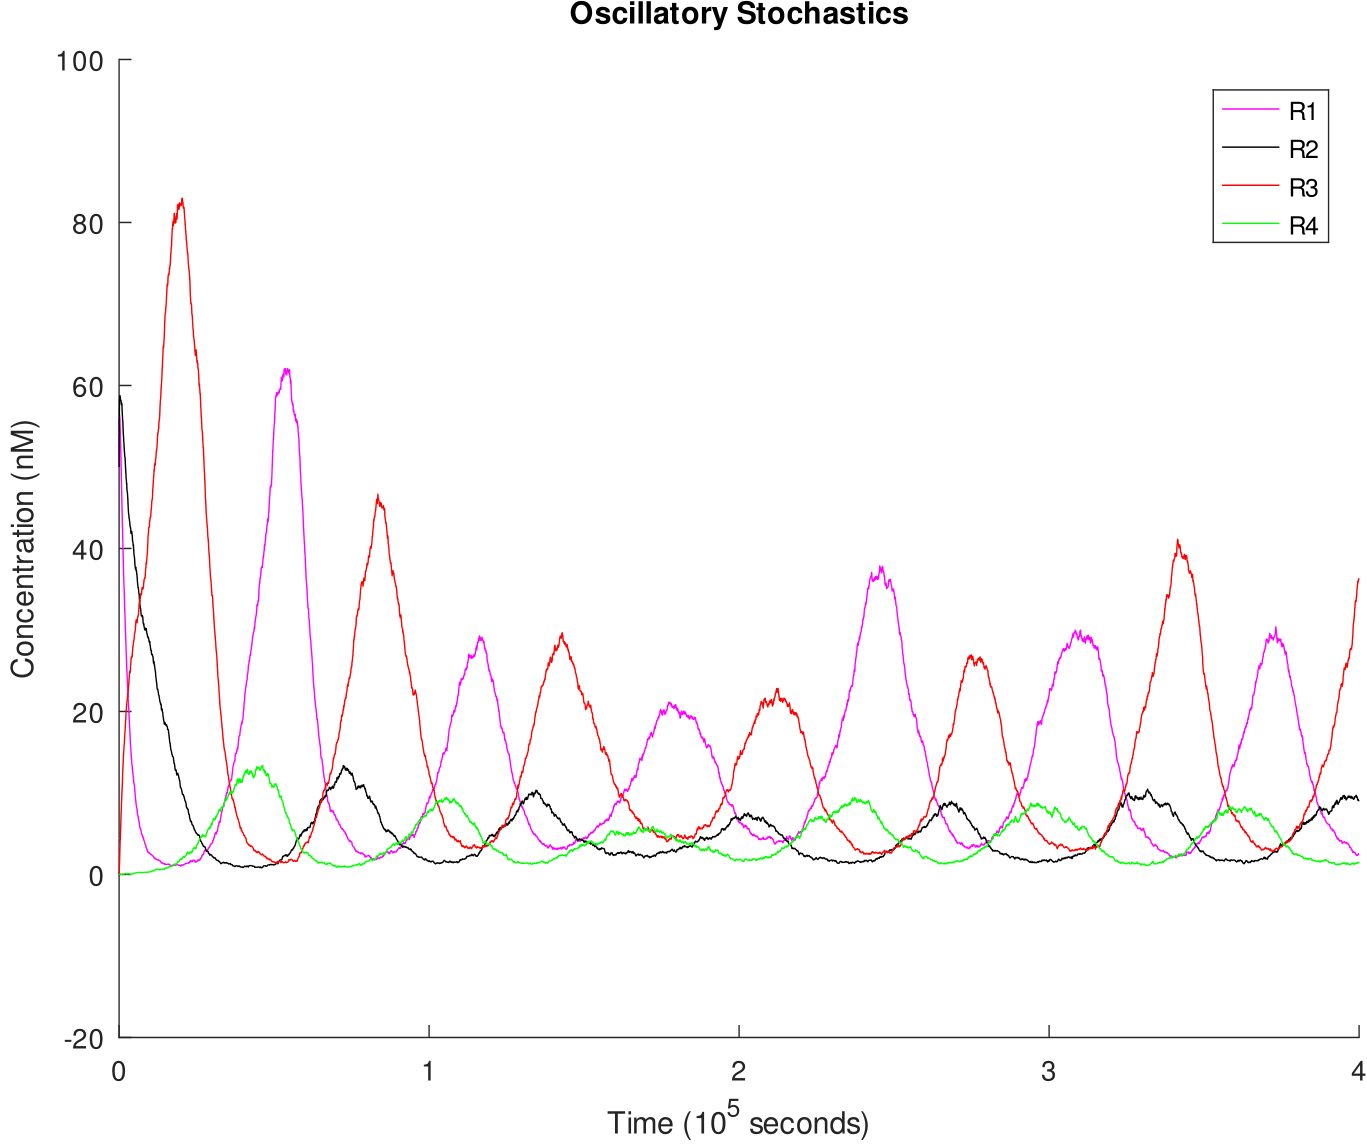
\includegraphics[width=0.55\textwidth]{stochastic-oscillator}
      \caption{\textbf{Effect of noise on oscillator function.} Input is set to \SI{5}{\nano M}, initial repressor state is $R1 = R2 = 50nM$, $R3 = R4 = 0nM$ and noise is scaled by $\frac{1}{55}$.}
      \label{fig.stochastic-oscillator}
    \end{figure}

    \begin{figure}[!htb]
      \centering
      \begin{subfigure}[t]{0.4\textwidth}
        \centering
        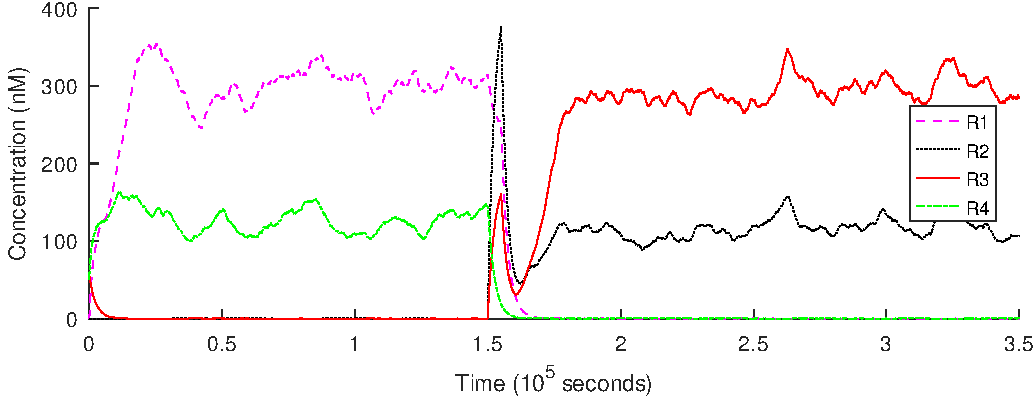
\includegraphics[width=\linewidth]{stochastic-switch-4}
        \caption{Initially, $R1 = R2 = 0nM$ and $R3 = R4 = 50nM$.}
        \label{fig.stochastic-switch-4}
      \end{subfigure}
      \hspace{2em}
      \begin{subfigure}[t]{0.4\textwidth}
        \centering
        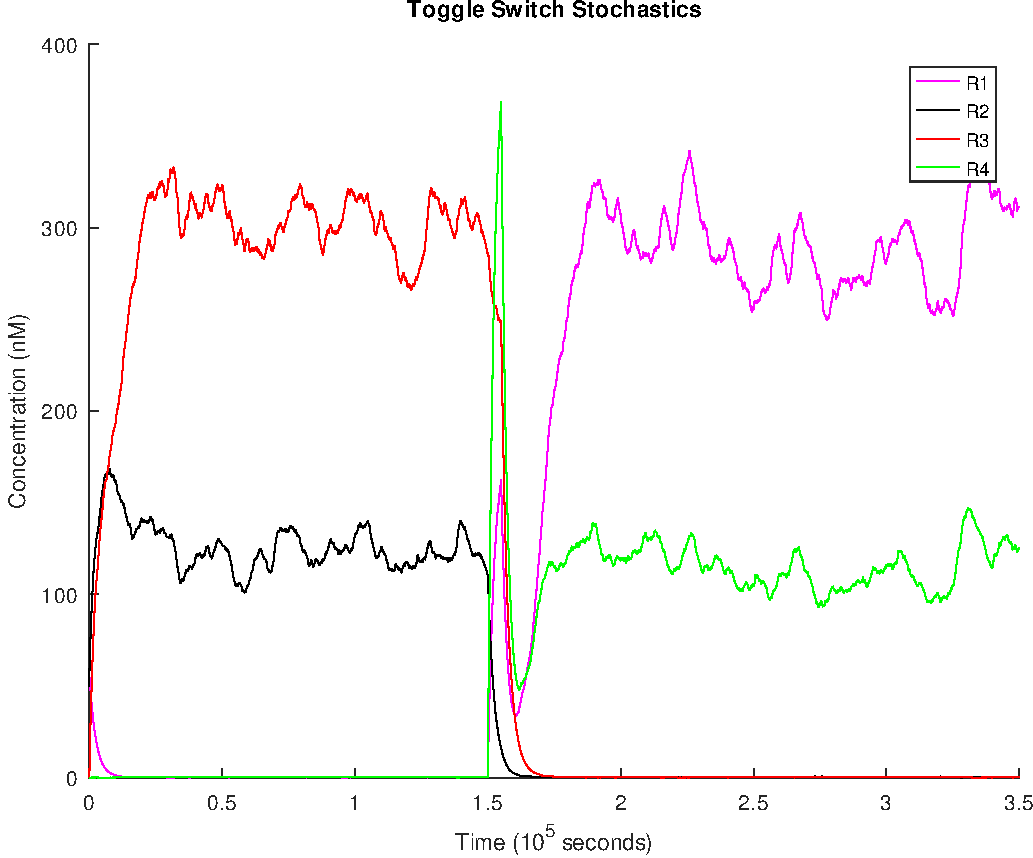
\includegraphics[width=\linewidth]{stochastic-switch-3}
        \caption{Initially, $R1 = R2 = 50nM$ and $R3 = R4 = 0nM$.}
        \label{fig.stochastic-switch-3}
      \end{subfigure}
      \caption{\textbf{Effect of noise on switching function.} Input is set to \SI{50}{\nano M} and random fluctuations are scaled by $\frac{1}{55}$.}
      \label{fig.stochastic-switch}
    \end{figure}

    \begin{figure}[!ht]
      \centering
      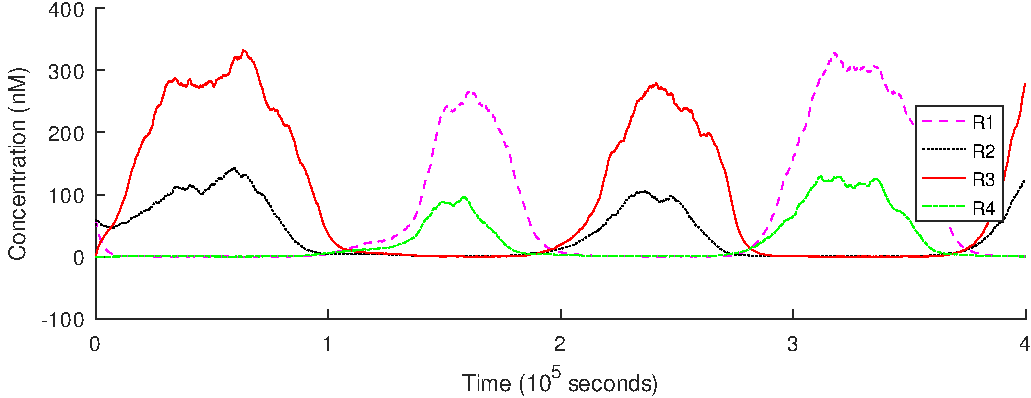
\includegraphics[width=0.55\textwidth]{stochastic-freqdiv-normal}
      \caption{\textbf{Usual frequency division behaviour.} Noise is scaled by $\frac{1}{55}$ and initial conditions are $R1 = R2 = 50nM$ and $R3 = R4 = 0nM$.}
      \label{fig.stochastic-freqdiv-normal}
    \end{figure}
    \begin{figure}[!hb]
      \centering
      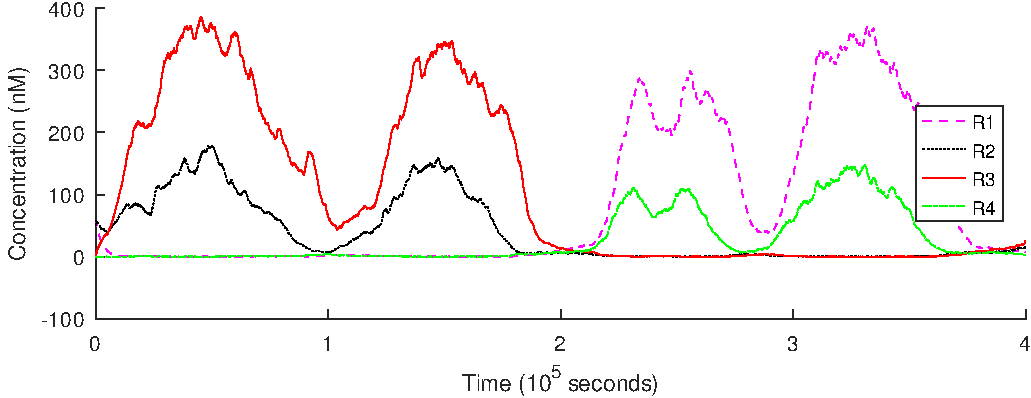
\includegraphics[width=0.55\textwidth]{stochastic-freqdiv-skip}
      \caption{\textbf{Irregular oscillations caused by stochastic fluctuations.} When noise is scaled by $\frac{1}{26}$, unintended behaviour is verified. Initial conditions are $R1 = R2 = 50nM$ and $R3 = R4 = 0nM$.}
      % scaling = 1/26
      % seed = 8.977812586558097e-01 # 2 red, 2 magenta
      % seed = 3.588309295243656e-01 # 4 red in a row
      \label{fig.stochastic-freqdiv-skip}
    \end{figure}

    We verified that among the three functionalities, frequency division possesses less robustness to intrinsic noise.
    During the stage where input is applied and proteins are all at a low concentration, random fluctuations may cause unintended oscillations as a pair of repressors rise in concentration and prevent transcription of the other two.
    An example of such irregular oscillating behaviour is given in Figure \ref{fig.stochastic-freqdiv-skip}.


\section{Conclusion}

  All operation modes in the multi-functional synthetic gene network were verified and to a large degree the results presented in \cite{originals} were replicated.
  It should be emphasised that the original work stands as an example of reproducible science, with detailed descriptions of model derivation, parameter decisions and extra experiments inside openly available supplementary material.
  Simplifications made using the \ac{qssa} to reduce the full \ac{ode} system proved being a good approximation as even though some small quantitative differences were observed, there was no impact on the network's qualitative dynamics.

  However, stochastic simulations would not provide the expected results without a significant reduction to noise variance.
  In fact, random fluctuations seem to be able to undermine the frequency division functionality to some degree.
  Additionally, the period-doubling bifurcation was empirically found to be at a much lower frequency than what is stated in the reference text.
  While this may have been a typographical mistake, it is a critical piece of information which can be used to know whether or not the model would work with existing or future oscillators.

  We highlight the idea that as synthetic networks grow in complexity and size, multi-functionality may arise more frequently and become difficult to avoid.
  While this can bring the benefits of reusable programmable components, it might also end up becoming a nuisance if models start behaving unexpectedly under the influence of certain inputs.
  At last, we believe further works should focus on a deeper exploration of parameter space.
  The motivation for this is double: it may allow for the characterisation of \textit{in vivo} implementation designs with reusable biological parts and will potentially verify the full set of specifications for this programmable genetic component and its multiple operating configurations.
